\documentclass[copyright,creativecommons]{eptcs-patched}

\usepackage{amsmath,amssymb}
\usepackage{graphicx}
\usepackage{url}
\usepackage{array}
\usepackage{hyperref}
\usepackage[strings]{underscore}
\usepackage{todonotes}
\usepackage{xspace}
\usepackage{color}
\usepackage{wrapfig}
\usepackage{listings}
\usepackage{enumitem
}

%%% COMMANDS %%%
\setcounter{tocdepth}{3}
\newcommand{\keywords}[1]{\par\addvspace\baselineskip
\noindent\keywordname\enspace\ignorespaces#1}

\newcommand{\blankline}{\vspace{\baselineskip}}
\newcommand{\halflineup}{\vspace{-0.5\baselineskip}}

% Names
\newcommand{\henshin}{\textsc{Henshin}\xspace}
\newcommand{\prism}{\textsc{PRISM}\xspace}
\newcommand{\groove}{\textsc{GROOVE}\xspace}
\newcommand{\cadp}{\textsc{CADP}\xspace}
\newcommand{\mcrl}{\textsc{mCRL}2\xspace}
\newcommand{\moment}{\textsc{MOMENT}2\xspace}
\newcommand{\maude}{\textsc{Maude}\xspace}

% Enable bold face in type writer font:
\DeclareFontShape{OT1}{cmtt}{bx}{n}{<5><6><7><8><9><10><10.95><12><14.4><17.28><20.74><24.88>cmttb10}{}

\definecolor{keyword}{RGB}{127,0,85}

\lstset{%
	% Keywords:
   keywords={sort,map,var,struct,eqn,forall,val,true,false,exists,act},
   keywordstyle={\color{keyword}\bfseries},
   emphstyle={\underbar},
	% Columns & spacing:
	columns=flexible,
	mathescape=true,
	% Styles
	basicstyle=\small\tt,
	commentstyle=\itshape\color{gray},
	texcl=true,
%	keywordstyle=\bfseries\color{black},
	frame=single,
	% Numbers
	numbers=left,
	numbersep=5pt
}

% mCLR2 listing style:
\lstnewenvironment{mcrlcode}[1][]{\lstset{#1}}{}

%%% TITLE %%%
\title{Instance-Aware Model Checking of Graph~Transformation~Systems using Henshin and mCRL2}

\def\titlerunning{Instance-Aware Model Checking of Graph Transformation Systems using Henshin and mCRL2}

\author{
Christian Krause
\and
Stefan Neumann
\and
\institute{Hasso Plattner Institute for Software Systems Engineering,
Prof.-Dr.-Helmert-Str. 2-3, D-14482 Potsdam, Germany}
\email{\{christian.krause|stefan.neumann\}@hpi.uni-potsdam.de}
}

\def\authorrunning{Christian Krause, Stefan Neumann}

\begin{document}

\maketitle


\begin{abstract}
Network topologies in distributed and mobile systems can be naturally described using graph-based models. Specifying configurations of such systems is realized by assigning nodes modeling entities in the network to logical locations in the graph. The operational semantics of such models can be formally described using graph transformation systems by modeling the interactive behavior of the entities in the network with rewrite rules. As an example, we model here the movement of autonomous railway shuttles along tracks and the creation of temporary convoys between shuttles.
%mobile device from one network cell to another, or creating temporary local connections between mobile devices. 

As a standard approach in formal methods, model checking facilitates the analysis of the dynamics modeled by graph transformation systems. However, in many settings such as in mobile and distributed systems, the model checking yields useful results only if it allows to reason about individual entities, e.g. specific railway shuttles, and their interactive behavior during the execution. Since the existing tools lack support for reasoning about individual entities, we introduce an approach and a toolchain for instance-aware model checking of graph transformation systems. We use \henshin as a modeling language and state space generation tool and \mcrl as model checking back-end.  
\end{abstract}



\section{Introduction}
\label{sec:introduction}

Graph transformation systems constitute a formal modeling approach for systems with structural state models and operational semantics that is defined in terms of rule-based rewriting of these models. Due to the graph-based nature of the state models, graph transformation is particularly well-suited to specify applications where the network topologies must be modeled explicitly, such as in distributed, mobile and reconfigurable systems (see, e.g.,~\cite{HGM06}). As a running example in this paper, we consider the RailCab system~\cite{RailCab} in which small, intelligent, autonomous shuttles provide on-demand passenger transfers. In our modeling, the shuttles operate on an existing and fixed railway network and share the tracks with other vehicles, e.g. trains. The dynamics of the system is defined using graph transformation rules that model the movement of vehicles on the tracks and the forming of convoys between shuttles.

As a standard approach in formal verification methods, finite graph transformation systems can be analyzed by constructing an explicit state space and applying model checking. However, the standard approach of using atomic propositions or simple transition labels for the model checking of graph transformation systems is rather unsatisfactory, since it does not provide a means to refer to entities in the structural state models. In this paper, we therefore describe an approach and a toolchain for \emph{instance-aware} model checking of graph transformation systems, which allows to refer to specific nodes in the graph models and to use quantification over node types in the specification of formulas. As technical contributions of this paper, we describe (1) our work on the state space generation tools for the graph transformation-based modeling language and toolset \henshin~\cite{henshin}, and (2) an adapter and user front-end which allows to automatically perform instance-aware model checking using the \mcrl~\cite{mcrl2} toolsuite.



% \bigskip
% 
% background info; motivation; case study; contributions: tool: state space generation + visualization + adapters for third-party model checker; particularly \mcrl for instance-ware model checking.
% 
% \vfill
% \paragraph{Organization} 
% In Section~\ref{sec:modeling} we describe the modeling in \henshin. In Section~\ref{sec:statespaces} we discuss the state space generation and vizualization tools in \henshin. In Section~\ref{sec:modelchecking-mcrl2} we present our approach for instance-aware model checking using an adapter for \mcrl. In Section~\ref{sec:modelchecking-other} we give an overview of other model checkers supported by \henshin. Section~\ref{sec:conclusions} contains conclusions and future work.

\newpage
\section{Modeling with \henshin}
\label{sec:modeling}

% Stereotypes
\newcommand{\action}[1]{\ensuremath{\langle\!\langle\mathsf{#1}\rangle\!\rangle}}

\henshin~\cite{henshin,henshin-website} is a modeling language and toolset that implements the double-pushout approach~\cite{Corradini97} for attributed typed graph transformation, based on structural data model in the Eclipse Modeling Framework~\cite{EMF}. Due to lack of space, we describe the relevant concepts only informally here. A \emph{graph transformation system} (GTS) consists of (1)~an (attributed) type graph, (2)~a set of parameterized\footnote{For a formal definition of graph transformation systems with parameterized rules see, e.g.,~\cite{HGM06}.} transformation rules, and (3)~a graph representing the initial state. Figure~\ref{fig:railcab} depicts the type graph and two parameterized transformation rules for modeling the RailCab system~\cite{RailCab} in \henshin.

\begin{figure}[t!]
\centering
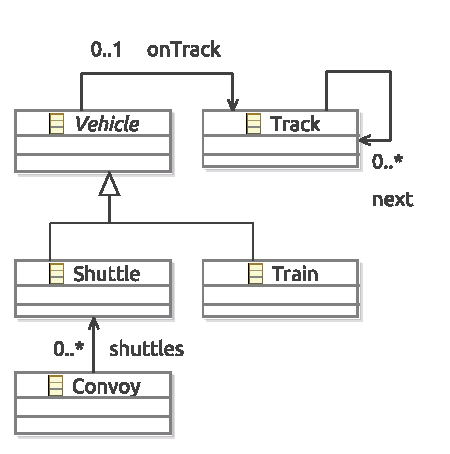
\includegraphics[width=4.7cm]{images/classes}\hspace{3mm}%
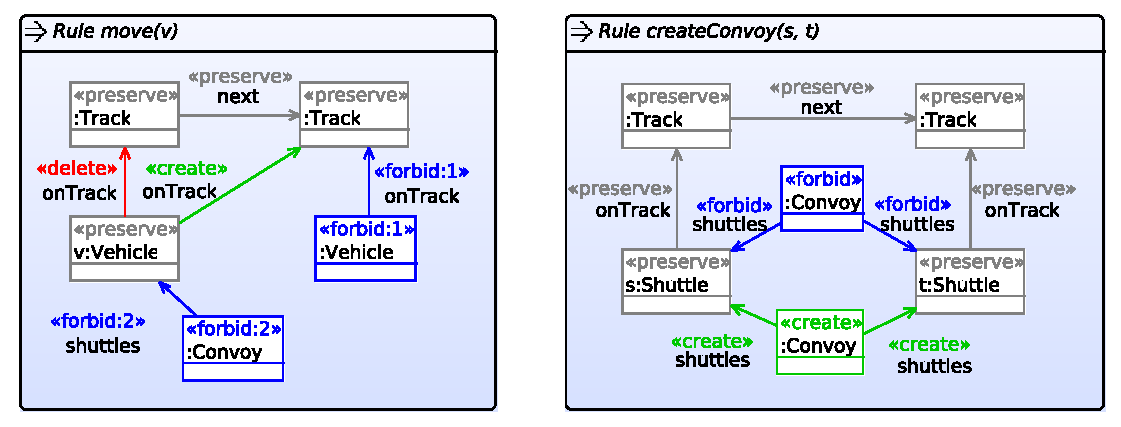
\includegraphics[width=11cm]{images/rules}
\vspace{-7mm}
\caption{Type graph (left) and transformation rules (mid and right) for the RailCab system in \henshin}
\label{fig:railcab}
\end{figure}

% System states in this approach are gioven by attributed typed graphs and the operational semantics is defined using parameterized graph rewrite rules..

\halflineup
\paragraph{(1) Type graph}
We distinguish five different node types: \textsf{Track}, \textsf{\textit{Vehicle}}, \textsf{Shuttle}, \textsf{Train} and \textsf{Convoy}. \textsf{\textit{Vehicle}} denotes an abstract node type and thus cannot be instantiated. \henshin supports node type inheritance which we use here to define \textsf{Shuttle} and \textsf{Train} as concrete realizations of \textsf{\textit{Vehicle}}. The edge type \textsf{next:Track}$\to$\textsf{Track} is used to model the topology of the railway system. The edge type \textsf{onTrack:\textit{Vehicle}}$\to$\textsf{Track} is used to specify the location of vehicles and \textsf{shuttles:Convoy}$\to$\textsf{Shuttle} models the existence of convoys between shuttles.

\definecolor{mygreen}{RGB}{0,200,0}
\definecolor{myred}{RGB}{200,0,0}
\definecolor{myblue}{RGB}{0,0,200}

\halflineup
\paragraph{(2) Parameterized transformation rules}
The parameterized transformation rules \textsf{\textit{move(v:Vehicle)}} and \textsf{\textit{createConvoy(s:Shuttle,t:Shuttle)}} in Figure~\ref{fig:railcab} are used here to model the operational semantics of the RailCab system. In the syntax of \henshin, rewrite patterns are denoted using the stereotypes \textcolor{darkgray}{\action{preserve}}, \textcolor{mygreen}{\action{create}}, \textcolor{myred}{\action{delete}} and \textcolor{myblue}{\action{forbid}}, respectively for matching and preserving, creating, deleting, and forbidding the existence of nodes or edges of a given type. The rule \textsf{\textit{move(v:Vehicle)}} moves the shuttle or train given by the parameter \textsf{\textit{v}} from its current track to one of its successor tracks. 
\begin{wrapfigure}{r}{3.3cm}
  \vspace{-5mm}
  \begin{center}
    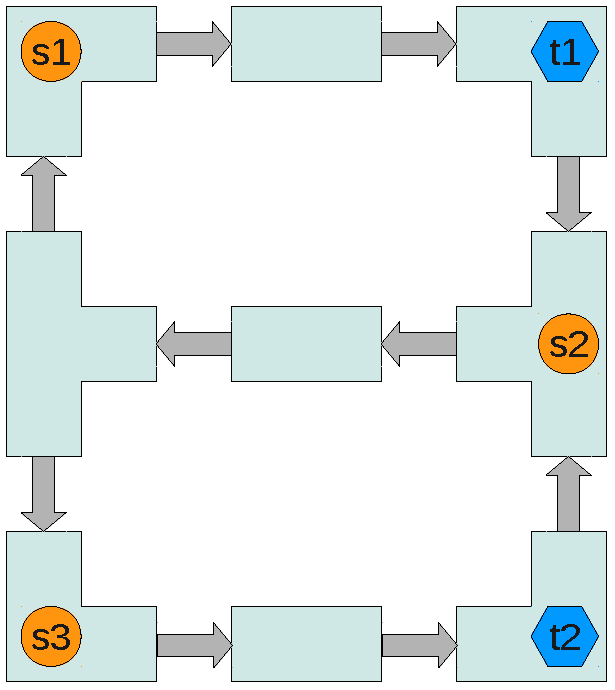
\includegraphics[width=3.25cm]{images/system}
  \end{center}
  \vspace{-5mm}
  \caption{Initial state}
  \label{fig:system}
  \vspace{-8mm}
\end{wrapfigure}
This is possible only if (1)~no other vehicle is on the next track, and (2)~the vehicle is currently not part of a convoy. The second constraint is added because modeling the movement of convoys is more involved and is for simplicity reasons not modeled here. The rule~\textsf{\textit{createConvoy(s:Shuttle,t:Shuttle)}} creates a convoy node between two shuttles which are located at adjacent tracks, if there is no convoy existing yet between them. We also introduce the rule~\textsf{\textit{deleteConvoy(s:Shuttle,t:Shuttle)}} which removes a convoy node again (not shown here).

\halflineup
\paragraph{(3) Initial state}
As initial state we use the typed traph which is schematically depicted in Figure~\ref{fig:system}. It consists of 9 interconnected tracks, 3 shuttles (depicted as circles) and 2 trains (depicted as hexagons) distributed on the tracks.

% A rule is a tuple $(r: L \rightharpoonup R)$
% A graph transformation system (GTS) is a pair $\langle P,G_0\rangle$ with $G_0$ an initial graph and $P$ a set of \emph{rules} of the form $p=\langle L,R,r,(C_i)_{i=1..n},(c_i)_{i=1..n}\rangle$ with $n\in \mathbb{N}$ where $L$ and $R$ are graphs called the left-hand side (LHS) and the right-hand side (RHS), $r : L \rightharpoonup R$ is a partial graph homomorphism, $\{C_i\}_{i=1..n}$ is a family of \emph{negative application conditions} (NACs) and $(c_i : L \to C_i)_{i=1..n}$ a family of total graph homomorphisms. For a graph $G$ a \emph{match} of a rule $p$ is a total graph homomorphism $m: L \to G$. Let $G'$ be the graph derived from $G$ by removing $m(L \setminus \mathit{dom}(r))$ and adding $R \setminus \mathit{codom}(r)$. Then $G \overset{r,m}{\Longrightarrow} G'$ is called a \emph{derivation}.

% \bigskip
% 
%  for NACs. Node inheritance: \textsf{Train} and \textsf{Shuttle} are specialization of the abstract type \textsf{Vehicle}. Graphical rule editor.
% High-level graphs: Structural data models\footnote{\ldots based on the Eclipse Modeling Framework}. Support for nested rules (amalgamation).
% 
% 
% Figure~\ref{fig:railcab} depicts two example rules for RailCab \cite{?}
% For simplicity, we do not model the movement of convoys. To avoid deadlocks, we also add a rule (note shown here) for removing a convoy again.


\section{State space generation and visualization with \henshin}
\label{sec:statespaces}

The \henshin toolset contains an interpreter engine implementing graph matching algorithms based on constraint solving for executing transformations. In addition, a number of tools for state space generation, visualization, and verification using invariant checking and model checking are included.

\begin{wraptable}{r}{5.3cm}
\vspace{-3mm}
\centering
\begin{tabular}{|c||r|r|r|}
\hline
IDs & States	& Trans. & Time \\ \hline\hline
no  & 1,274		& 4,297  & 1s \\ \hline
yes & 15,030	& 51,384 & 20s \\ \hline
\end{tabular}
\caption{RailCab LTS details}
\label{tab:details}
\vspace{-3mm}
\end{wraptable}
\halflineup\paragraph{State space generation}
State spaces are generated as labeled transition systems (LTSs) where the states are graphs. 
Two different modes are supported: without and with nodes IDs. In the mode without node IDs, transition labels consist only of rule names, without parameters. In this mode, states are compared using mere graph isomorphy checking and thus, different instances of the same node type cannot be distinguished. In the mode with node IDs, all nodes whose type occurs as a parameter type in a rule, get a unique ID, e.g. all nodes of type \textsf{Train} and \textsf{Shuttle} in the RailCab example. These node IDs are then used as identifiers in the parameters of transition labels. The mode with node~IDs yields  significantly larger state spaces. However, it is required to distinguish between different nodes of the same type and to track their history, which is a key ingredient for the instance-aware model checking as we argue in Section~\ref{sec:modelchecking-mcrl2}.
The sizes of the generated LTSs for the RailCab example without and with node IDs are shown in Table~\ref{tab:details} together with the time required for generating the complete state spaces.\footnote{The tests were conducted on a 64-bit Intel(R) Xeon(R) CPU with 4$\times$2.50GHz and 8GB memory
running Linux 2.6.26.} \henshin also supports interactive visualization and exploration of small state spaces (for $\sim\!10^4$ states).


\halflineup\paragraph{Optimizations}
The state space generation tool is based on a memory-efficient state space model and makes extensive use of caching. On multi-core processors, the state space generation is performed using multiple threads. The state space generation is implemented as a hybrid approach of depth-first and breadth-first search.\footnote{Depth-first search can make better use of caching, but cannot be parallelized. Therefore, the tool unfolds a fixed number of new states at once using multiple threads. Thus, the tool implements a hybrid approach of depth-first and breadth-first search.} Indexing of states is crucial to avoid unnecessary isomorphy checks and is implemented using a graph hash function. For the graph isomorphy checking, the rule match finding engine of the \henshin interpreter is used. Node IDs are generated only for those nodes whose type is used as a parameter in a rule. Thereby, symmetries in the underlying system topology can be used to reduce the size of the state space. For instance, in the RailCab example the topology of the track network can be mirrored vertically (see Figure~\ref{fig:system}), which reduces the size of the state space by a factor of~2.


\section{Instance-aware model checking with \mcrl}
\label{sec:modelchecking-mcrl2}

\mcrl~\cite{mcrl2} is a behavioral specification language and associated toolset with support for model checking based on the modal $\mu$-calculus extended with regular expressions, data and time~\cite{GM99}. \mcrl can indirectly model check explicit state spaces as generated by \henshin using the import tool \texttt{lts2lps} which converts a given LTS into \mcrl's own format (so-called \emph{linear process specifications}). 

The \henshin state space tools include an adapter and a front-end for instance-aware model checking of generated state spaces using \mcrl. State spaces are first converted into an LTS format readable by \mcrl. In the mode with node IDs, the adapter extracts all used node IDs from the state space first and generates a data type definition in the format of \mcrl. For the RailCab example, the generated data type specification is shown in Listing~\ref{mcrl2data}. As data types in \mcrl cannot make use of inheritance, the adapter identifies \textsf{Vehicle} as common supertype of \textsf{Shuttle} and \textsf{Train}. The adapter found five node IDs for this type and generates the data type \texttt{\underline{Vehicle}} accordingly as a sum over five different identifiers, modeling the instances. These identifiers are also used in the parameters of the transitions and can be therefore used for the model checking (see also the generated actions and their parameter types in line~2). The adapter also generates the helper predicates \texttt{isShuttle} and \texttt{isTrain} (see line 4--5) which can be used to check for the real data type of instances in formulas. 

Using the generated LTS and data type definition in Listing~\ref{mcrl2data}, we can now directly verify $\mu$-calculus formulas with data using \mcrl. For our running example we check the following two properties:

\lstset{emph={Vehicle,Bool}}

\begin{mcrlcode}[float=t,aboveskip=-1mm,belowskip=-1mm,
  caption={Generated \mcrl data type specification for the RailCab example},label={mcrl2data}]
sort Vehicle = struct s1 | s2 | s3 | t4 | t5;
act move : Vehicle;    createConvoy : Vehicle#Vehicle;    deleteConvoy : Vehicle#Vehicle;
var x : Vehicle;
map isShuttle : Vehicle -> Bool;       eqn isShuttle(x) = (x==s1) || (x==s2) || (x==s3);
map isTrain : Vehicle -> Bool;         eqn isTrain(x) = (x==t4) || (x==t5);
\end{mcrlcode}
\begin{mcrlcode}[float=t,,aboveskip=0mm,belowskip=-2mm,
  caption={Example property \emph{a)}},label={propA}]
forall s:Vehicle.val(isShuttle(s)) => 
 ([true*] (exists t:Vehicle.val(isShuttle(t)) && (<true*.createConvoy(s,t)> true)))
\end{mcrlcode}

%\vspace{-8mm}
%\begin{mcrlcode}[float=h,caption={Example property B},label={propB}]
%forall s:Vehicle.val(isShuttle(s)) => 
% ([true*] (exists t:Vehicle.val(isShuttle(t)) && (<move(s)*.createConvoy(s,t)> true)))
%\end{mcrlcode}

\begin{enumerate}[label=\emph{\alph*})]
  \item For every shuttle it holds in every state that it can eventually form a convoy with another shuttle.
	In \mcrl-syntax, the property can be written as shown in Listing~\ref{propA}.
	This property is satisfied.
  \item For every shuttle it holds in every state that it can eventually form a convoy with another shuttle 
  only by moving itself (meaning that no other vehicle stands in the way). We can adapt the formula in Listing~\ref{propA} by replacing \lstinline!<true*.createConvoy(s,t)>! with \lstinline!<move(s)*.createConvoy(s,t)>!.
  This property is not satisfied, meaning that it is possible that a train blocks a shuttle.
\end{enumerate}
Note that this approach allows us to use existential and forall-quantification over node types in the original graph transition system and to track transitions involving bound node variables.


\section{Other model checkers supported by \henshin}
\label{sec:modelchecking-other}

\paragraph{OCL invariants}
The Object Constraint Language (OCL)~\cite{ocl} can be used in \henshin to specify and check structural state invariants. For small state spaces, found counterexamples are highlighted in the state space explorer and can be inspected in more detail.
 
\halflineup\paragraph{\cadp}
Besides \mcrl, model checking of modal $\mu$-calculus formulas for explicit state spaces, e.g., given as LTSs, is also supported by the the \cadp toolsuite~\cite{cadp}. The \henshin state space tools include an adapter which translates state spaces generated from graph transformation systems into the input format of \cadp, and invokes the \texttt{evaluator} model checking tool. In contrast to \mcrl, \cadp can output counterexamples which are automatically extracted and --if possible-- shown in the graphical state space explorer. However, \cadp can currently not be used for instance-aware model checking.
 
\halflineup\paragraph{\prism}
Based on the approach of stochastic graph transformation~\cite{HGM06}, \henshin rules can be annotated with stochastic delays (formally, rates of exponential distributions). The rates together with the generated state space give rise to a Continuous Time Markov Chain. The \henshin state space tools can generate such a stochastic model in the input format of the \prism model checker. Using a front-end in the state space explorer, the steady state probabilities can be computed, formulas
specified in Continuous Stochastic Logic (CSL) %~\cite{BHHK00}
can be verified, and plots can be generated using \prism.

% WICHTIGSTEN SACHEN MERGEN MIT DEM OBEREN TEIL. DANN HIER NUR NOCH ZUSAETZLICHE FEATURES UND AVAILABILITY OF THE TOOL
% 
% GENERAL TOOL OVERVIEW -- UPDATE!!! 
% We interpret EMF instance models as states
% and rule applications as transitions which are labeled with
% the name of the applied rule. Provided with one or more
% initial state models, this gives rise to a labeled
% transition system which can be model checked.
% We have implemented this state space analysis approach in a
% graphical environment as part of the Henshin
% toolset~\cite{henshin-website}. Our tool (shown in
% Fig.~\ref{fig:tool}) supports efficient state space
% generation, the use of abstractions, state space
% visualization, and model checking using third-party~tools.

%\begin{figure}
%\centering
%\setlength\fboxsep{0pt}
%\setlength\fboxrule{0.5pt}
%\fbox{\includegraphics[width=\textwidth]{images/tool}}
%\caption{NEU, WENN UEBERHAUPT. screenshot of the Henshin state space explorer}
%\label{fig:tool}
%\vspace{-3mm}
%\end{figure}

% \paragraph{State space generation}\ldots
% graph hash functions\ldots 
% Optimization for graph isomorphy checking for graph transformation systems with fixed topologies such as the RailCab example. Idea: statically check which parts types of elements cannot be changed by the rules. Based on the containment tree structure in EMF models, we can precompute a partial match for these elements and use it for the isomorphy checking. SPEEDUP fuers BEISPIEL??
% 
% \paragraph{State space visualization}\ldots
% 
% UPDATE!!!
% A core functionality of our state space analysis tools is
% the generation of an explicit state space, which can be done
% in a graphical state space explorer or `off\-line', which is
% more efficient. States are represented by an index and
% additionally contain a hash value of the EMF model they
% represent, which allows efficient lookup of states given an
% arbitrary EMF model.
% Note that in a state space, links to the
% models are stored only for the initial states. The models of
% all other states are derived at runtime and cached only. A
% flag associated with the states indicates whether they are
% already unfolded or not, allowing to resume the 
% state space generation at a later point. Our underlying
% state space implementation is itself based on an EMF model.
% For efficient storage, we use a custom binary file format,
% which can also be exported to standard LTS formats.
% Moreover, on multi-core machines, the state space generation 
% is done using multiple worker threads.
% However, this requires to lock the whole state space for
% checking whether a generated model is already represented by
% a state and adding a new state if it is unknown. Since the
% lookup of states requires a possibly expensive equality
% check of state models, we removed the locking for the state
% lookup phase and added a monitoring for concurrently 
% occurring state space modifications. Using this
% optimization, the state space needs to be locked only 
% for comparison with the states that have been added
% by other worker threads during the lookup phase. Initial
% experiments showed that the multi-threaded implementation
% can indeed increase the performance of the state space
% generation significantly. For instance, in our dining
% philosophers example without the use of any abstractions,
% the multi-threaded implementation was approximately
% 2.6~times faster on a machine with 4 cores. 
% Using the lightweight state space model and
% multi-threaded state space generation, our 
% tool can handle state spaces with millions of
% states on recent desktop computers, depending on
% the size of the models.
% Moreover, small state spaces can be visualized in a
% graphical state space explorer, 
% as shown in Fig.~\ref{fig:tool}. This tool supports animated
% layouting using a force-based (spring) algorithm and export
% to \LaTeX. Moreover, instance models of initial and
% derived states can be inspected.
% 
% \paragraph{Configurable isomorphy checks}
% 
% UPDATE!!! NICHT ZU TECHNISCH! 
% The lookup of states during the state space generation
% is done using hash values and a standard equality
% check for EMF models. References between objects in 
% EMF are stored and compared as lists. However, in our
% graph-based transformation approach, the order of references
% is not considered. Therefore, switching from the EMF-based
% equality check to a graph isomorphism check yields a
% bisimulation-preserving abstraction of the original state
% space, which prevents an exponential blowup. Note that
% the used hash function needs to be adapted,~too.
% Moreover, if none of the rules defines an application
% condition on the objects' attributes, the values of all
% attributes can be ignored as well in the equality
% check and the hash value calculation, which yields another
% bisimulation-preserving abstraction. Note that rules
% can be analyzed statically to determine whether they contain
% attribute conditions or not. Ensuring bisimulation
% equivalence of the abstract state space is particularly
% important for applying model checking, as discussed in
% Section~\ref{sec:model-checking}. The two abstractions
% mentioned above are both implemented in the state space
% analysis tools in Henshin and can be enabled
% in the state space explorer, as shown in
% the right part of Fig.~\ref{fig:tool}.
% 
% TABELLE MIT VERGLEICH DER VERSCHIEDENEN VARIANTEN: Zustaende, Transitionen, (Zeit ?)
% 
% \paragraph{Invariant Checking}
% The Object Constraint Language (OCL)~\cite{ocl} can be used
% to specify structural properties of EMF models. In Henshin,
% OCL is supported for validating structural invariants
% in state spaces. Found counterexamples are highlighted in
% the state space explorer and can be inspected in more
% detail.
% 
% \paragraph{Model checking}
% 
% State space generation, abstraction and visualization is
% implemented directly in Henshin. Model checking, however,
% is not done by Henshin itself. Instead, third-party model
% checkers and other analysis tools are used to validate
% structural and behavioral properties. The Henshin state
% space explorer provides a uniform front-end to a number
% of analysis tools, as discussed in the following.
% 

\section{Related approaches and tools}
\label{sec:relatedwork}

In the \moment~\cite{Boronat2009} tool, verification of graph transformation systems
%is implemented using rewriting logic in \maude~\cite{maude}. Formal analysis 
is supported using OCL invariant checking and LTL model checking. To distinguish between different instances of the same type in an LTL formula, node identities must be encoded using ID-attributes which must be defined already in the initial state. Thus, only nodes which are already included in the start graph can be distinguished in the model checking. To the best of our knowledge, existential and forall-quantification over node types are also not supported.
%
Another tool for LTL and CTL model checking of graph transformation systems is \groove~\cite{rensink06}. Model checking in \groove is based on atomic propositions which are defined using graph patterns. An atomic proposition is fulfilled for a given state graph iff the pattern can be matched. Therefore, it is not possible to reason about specific instances or to quantify over node types.

% Skip??
% 
% , whereas Henshin 
% supports the full expressiveness of EMF for state models,
% including containment references. \groove supports model
% checking of LTL and CTL formulas, Henshin allows to
% use the more expressive modal $\mu$-calculus using CADP and
% \mcrl. \groove itself does not support probabilistic model
% checking and also does not integrate with PRISM. However,
% a toolchain for stochastic analysis of graph grammars
% defined in \groove is considered in~\cite{HGM06}.
% Henshin supports two
% bisimulation-preserving abstractions using graph
% isomorphism checking and attribute abstraction. 
% The former is also supported by
% \groove. Moreover, \groove can handle infinite state spaces
% using so-called shape graphs. However, this abstraction is
% not bisimulation-preserving.
% 
% AGG~\cite{Taentzer04} is a modeling and verification tool for
% attributed graph grammars with support for critical pair
% analysis~\cite{HKT02} and termination checks~\cite{EE05}.
% Similarly to GROOVE, AGG is based on graphs and cannot model
% containment references of EMF models. Therefore, AGG's
% analysis tools cannot be applied to EMF model
% transformations in general.




%A distributed state space generation scheme for GROOVE is
%presented in~\cite{Kant10}. It uses the
%LTSmin~\cite{ltsmin} toolset for 
%\nocite{Kant10}


%\halflineup
\section{Conclusions and future work}
\label{sec:conclusions}

We have introduced an approach and a toolchain for instance-aware model checking of graph tranformation systems using \henshin and \mcrl, which increases the expressiveness of model checking for graph transformation systems by allowing to refer to specific instances and to quantify over node types. As future work, we plan to use \cadp as model checking back-end (since it supports counterexample extraction), and to investigate ways to accommodate for the increased state space sizes.
%\halflineup

% \paragraph{Notes on the \henshin Toolset} The graphical editor for rules in \henshin as shown in Figure~\ref{fig:railcab}, the state space generation and visualization as presented in Section~\ref{sec:statespaces} and the adapter for \mcrl and the other model checkers as presented in Section~\ref{sec:modelchecking-mcrl2} and~\ref{sec:modelchecking-other} was implemented by the first author of this paper.

%\paragraph{Acknowledgments} The authors are grateful to the \mcrl development team for their support.

\bibliographystyle{eptcs}
\bibliography{henshin_mcrl2}

\end{document}
